\subsection{古典補償器の設計}

補償器設計は、要求仕様を開ループ $L(s)=C(s)G(s)$ の形へ翻訳する作業である。位相余裕を増やしたいなら進み補償、低周波ゲインを増やして定常偏差を減らしたいなら遅れ補償、両方必要なら遅れ進み補償を使う。

\begin{definition}[進み補償]
\begin{equation}
  C_{lead}(s)=K\frac{1+Ts}{1+\alpha Ts},
  \qquad 0<\alpha<1
\end{equation}
を進み補償という。零点が極より低い周波数にあるため、ある周波数帯で正の位相を加える。
\end{definition}

最大位相進みは
\begin{equation}
  \phi_{max}=\sin^{-1}\frac{1-\alpha}{1+\alpha}
\end{equation}
であり、その周波数は
\begin{equation}
  \omega_m=\frac{1}{T\sqrt{\alpha}}
\end{equation}
である。設計では、必要な位相余裕の不足分に安全余裕を足し、$\alpha$ を決め、望むゲイン交差周波数を $\omega_m$ 付近へ置くように $T$ を決める。

\begin{definition}[遅れ補償]
\begin{equation}
  C_{lag}(s)=K\frac{1+Ts}{1+\beta Ts},
  \qquad \beta>1
\end{equation}
を遅れ補償という。低周波ゲインを相対的に上げ、定常偏差を小さくするために使う。
\end{definition}

遅れ補償は位相を少し遅らせるので、ゲイン交差周波数の近くに置くと安定余裕を悪くする。したがって、折点はゲイン交差周波数より十分低く置き、低周波の精度改善を主目的にする。

\subsection{フィードフォワード、カスケード制御、外乱オブザーバ}

閉ループ制御は、測定した偏差を使って未知の誤差を修正する構造である。一方、目標値の変化、加速度指令、荷重、流量、周囲温度のように、制御対象へ加わる信号の一部があらかじめ分かっている場合がある。この既知情報を偏差が現れる前に操作量へ入れる方法をフィードフォワード制御という。フィードフォワードはフィードバックの代わりではない。モデルが正しい範囲で必要入力を先に出し、モデル誤差、未知外乱、初期値ずれをフィードバックで補正する構成である。

\subsubsection{既知目標値と既知外乱からのフィードフォワード}

まず、対象を
\begin{equation}
  y=G(s)u+G_d(s)d
\end{equation}
で表す。$u$ は操作量、$d$ は外乱、$G_d$ は外乱から出力までの伝達関数である。外乱 $d$ が測定または予測でき、その測定値を $d_m$ とする。フィードバック制御器を $C(s)$、外乱フィードフォワードを $F_d(s)$ として
\begin{equation}
  u=C(s)(r-y)+F_d(s)d_m
\end{equation}
を入れる。$d_m=d$ と仮定して代入すると
\begin{align}
  y&=G\{C(r-y)+F_d d\}+G_d d,\\
  (1+GC)y&=GCr+(GF_d+G_d)d,
\end{align}
したがって
\begin{equation}
  y=\frac{GC}{1+GC}r+
  \frac{GF_d+G_d}{1+GC}d
\end{equation}
である。名目モデル $G_n,G_{d,n}$ が正しく、$G_n^{-1}G_{d,n}$ が安定でプロパーに実装できるなら
\begin{equation}
  F_d(s)=-G_n(s)^{-1}G_{d,n}(s)
\end{equation}
と選ぶことで、名目上は $GF_d+G_d=0$ となり、外乱項が消える。外乱が対象入力にそのまま加わる入力外乱では $G_d=G$ なので、理想的な補償は単に $F_d=-1$ である。これは、既知の入力外乱と反対向きの入力を先に加えるという意味である。

目標値に対しても同じ考え方を使える。名目対象 $G_n$ に対し、望ましい目標値応答を安定でプロパーな伝達関数 $M(s)$ として与える。開ループの必要入力を
\begin{equation}
  u_{ff}=F_r(s)r,
  \qquad
  F_r(s)=G_n(s)^{-1}M(s)
\end{equation}
とすれば、名目上は $y=M r$ になる。ただし、この式がそのまま使えるとは限らない。$G_n$ に右半平面零点やむだ時間があると、安定な因果系として正確な逆系を作れない。相対次数が大きい対象では $G_n^{-1}M$ がプロパーでなくなることもある。このため、実装では $M$ を十分遅くし、必要なら低域通過フィルタを加え、入力飽和を越えない範囲で近似逆を使う。

フィードフォワード設計で明示すべき仮定は三つである。第一に、既知信号 $r$ または $d_m$ が制御計算に間に合う時点で利用でき、正しい単位と符号を持つこと。第二に、名目モデルの逆を使う周波数帯で、零点、むだ時間、未モデル化高周波動特性が無視できること。第三に、フィードフォワード入力を加えてもアクチュエータが飽和しないことである。これらが崩れると、偏差が小さくなるどころか、誤った先回り入力によってフィードバックが補正すべき誤差を増やしてしまう。

\subsubsection{二自由度構造としての解釈}

一自由度の負帰還では、同じ制御器 $C$ が目標値追従と外乱抑制の両方を決める。これに対し、目標値から入力への経路と、測定値から入力への経路を分けて
\begin{equation}
  u=C_r(s)r-C_y(s)y
\end{equation}
と書く構造を二自由度制御構造という。対象入力に外乱 $d_i$ が加わる場合、
\begin{align}
  y&=G(u+d_i),\\
  u&=C_r r-C_y y
\end{align}
であるから
\begin{align}
  y&=G(C_r r-C_y y+d_i),\\
  (1+GC_y)y&=GC_r r+Gd_i.
\end{align}
したがって
\begin{equation}
  y=\frac{GC_r}{1+GC_y}r+
  \frac{G}{1+GC_y}d_i
\end{equation}
となる。分母 $1+GC_y$ は、閉ループ極、安定余裕、外乱抑制、測定ノイズの入り方を決める。一方、$C_r$ は主に目標値から出力までの分子を変える。つまり、$C_y$ でロバスト性と外乱抑制を確保し、$C_r$ または $F_r=C_r-C_y$ で目標値応答を整える、という役割分担ができる。

後で扱う二自由度 PID は、この構造の実装例である。比例項と微分項に目標値重みを入れると、測定値側のフィードバックを保ったまま、目標値ステップに対する比例キックや微分キックを弱められる。ただし、二自由度化しても閉ループ安定性の基本は $1+GC_y$ に残る。目標値経路だけを滑らかにしても、出力外乱やモデル誤差への性質が自動的に改善するわけではない。

\subsubsection{カスケード制御と帯域分離}

一つの制御対象の中に、速く測れる内部量と、遅く制御したい外部量がある場合は、制御ループを内側と外側に分ける。これをカスケード制御という。入力 $u$ から内部量 $z$ までの伝達関数を $G_i$、内部量 $z$ から出力 $y$ までの伝達関数を $G_o$ とする。
\begin{equation}
  z=G_i(u+d_i),
  \qquad
  y=G_o z
\end{equation}
内側制御器 $C_i$ が $z$ を目標値 $z_r$ に追従させ、外側制御器 $C_o$ が $z_r$ を作る。
\begin{equation}
  u=C_i(z_r-z),
  \qquad
  z_r=C_o(r-y)
\end{equation}
内側閉ループの感度と相補感度を
\begin{equation}
  S_i=\frac{1}{1+G_iC_i},
  \qquad
  T_i=\frac{G_iC_i}{1+G_iC_i}
\end{equation}
とおくと、
\begin{align}
  z&=T_i z_r+G_iS_i d_i,\\
  y&=G_oT_i z_r+G_oG_iS_i d_i.
\end{align}
外側ループに対する等価制御対象は $G_oT_i$ である。内側ループの帯域幅を $\omega_{b,i}$、外側ループの帯域幅を $\omega_{b,o}$ とすると、外側設計の周波数範囲で
\begin{equation}
  T_i(j\omega)\simeq 1,
  \qquad
  \angle T_i(j\omega)\simeq 0
  \quad
  (0\leq\omega\leq \omega_{b,o})
\end{equation}
となるように、通常は
\begin{equation}
  \omega_{b,i}\geq 3\omega_{b,o}
\end{equation}
を最低条件とし、余裕があれば $5$ 倍から $10$ 倍程度の分離を取る。内側ループが十分速ければ、外側ループは $z$ がほぼ指令通りに動くものとして設計できる。また、$G_iS_i d_i$ が小さくなるため、入力側や内部側の外乱は外側へ伝わる前に抑えられる。

カスケード制御が有効であるためには、内部量 $z$ を測定できること、内側アクチュエータが外側の要求より速く動けること、内側ループ単独で安定余裕を持つことが必要である。内側に強いノイズ、量子化、むだ時間がある場合、帯域を上げるほど外側へ位相遅れとノイズが入る。さらに、内側が飽和すると外側制御器は「内部量が追従している」という前提を失うため、外側の積分器にもアンチワインドアップを入れる必要がある。

\subsubsection{外乱オブザーバの基本構成}

外乱が測れない場合でも、名目モデルを使って「入力から予測される出力」と「実際の出力」の差から外乱を推定できることがある。この考え方を外乱オブザーバという。ここでは、外乱 $d$ が対象入力に加わる
\begin{equation}
  y=P(s)\{u+d\}
\end{equation}
という形を考える。名目モデルを $P_n(s)$ とし、低域通過フィルタを $Q(s)$ とする。外乱推定値を
\begin{equation}
  \hat{d}=Q(s)\{P_n(s)^{-1}y-u\}
\end{equation}
で作り、補償後の入力を
\begin{equation}
  u=u_0-\hat{d}
\end{equation}
とする。もし $P=P_n$ なら、
\begin{align}
  P_n^{-1}y-u
  &=P_n^{-1}P_n(u+d)-u\\
  &=d
\end{align}
なので
\begin{equation}
  \hat{d}=Qd
\end{equation}
である。したがって対象へ入る合計入力は
\begin{equation}
  u+d=u_0+(1-Q)d
\end{equation}
となる。低周波で $Q(j\omega)\simeq 1$ なら、その帯域の外乱はほぼ打ち消される。高周波で $Q(j\omega)\simeq 0$ とすれば、センサノイズや未モデル化動特性を逆モデルで増幅することを避けられる。

外乱オブザーバでは $Q$ フィルタの選択が中心である。$Q(0)=1$ として定常外乱を推定し、遮断周波数を上げるほど外乱抑制帯域は広がる。しかし $P_n^{-1}$ は高周波で大きなゲインを持ちやすく、相対次数のためにプロパーでないこともある。このため、$Q P_n^{-1}$ がプロパーで安定になるように、$Q$ の次数を十分高くする。名目モデルが右半平面零点やむだ時間を持つ場合、厳密な安定逆は作れないので、最小位相部分だけを反転する近似逆を使う。さらに、外乱オブザーバはモデル誤差を外乱として扱うため、$Q$ の帯域を未モデル化共振やサンプリング周波数に近づけすぎると、かえって閉ループを不安定化する。

\begin{example}[DC モータ速度制御における構成例]
DC モータの角速度を $\omega$、電流を $i$、電圧を $v$、負荷トルクを $\tau_L$ とする。単純化したモデルは
\begin{align}
  J\dot{\omega}+b\omega&=K_t i-\tau_L,\\
  L\dot{i}+Ri&=v-K_e\omega
\end{align}
である。電流は速度より速く測定・制御できることが多いため、内側に電流ループ、外側に速度ループを置く。内側電流ループの帯域を速度ループの少なくとも数倍にすれば、外側からは
\begin{equation}
  i\simeq i_r
\end{equation}
と近似できる。

望ましい速度軌道 $\omega_r(t)$ と既知の負荷トルク測定値 $\tau_{L,m}$ があるなら、機械式から必要電流のフィードフォワードを
\begin{equation}
  i_{ff}=
  \frac{J_n\dot{\omega}_r+b_n\omega_r+\tau_{L,m}}{K_{t,n}}
\end{equation}
と計算できる。速度制御器を $C_\omega$ とすれば、外側の電流指令は
\begin{equation}
  i_r=i_{ff}+C_\omega(s)(\omega_r-\omega)
\end{equation}
である。ここで $J_n,b_n,K_{t,n}$ は名目値である。フィードフォワードは加速に必要なトルクと粘性損失、既知負荷を先に補い、速度フィードバックは残った誤差だけを修正する。

負荷トルクが測れない場合は、電流からトルク入力 $\tau_m=K_{t,n}i$ を作り、機械部の名目モデル
\begin{equation}
  P_n(s)=\frac{1}{J_ns+b_n}
\end{equation}
を用いる。入力外乱を $d=-\tau_L$ と定義すると、
\begin{equation}
  \hat{d}=Q(s)\{P_n(s)^{-1}\omega-\tau_m\}
\end{equation}
は低周波で $-\tau_L$ を推定する。したがって
\begin{equation}
  i_r=
  \frac{J_n\dot{\omega}_r+b_n\omega_r-\hat{d}}{K_{t,n}}
  +C_\omega(s)(\omega_r-\omega)
\end{equation}
とすれば、$-\hat{d}$ が負荷トルク補償として働く。この設計では、電流ループが十分速いこと、速度センサのノイズが $Q P_n^{-1}$ で過度に増幅されないこと、電圧と電流の飽和を越えないことを確認する必要がある。
\end{example}

\subsection{PID を実装として設計する}

PID は伝達関数として
\begin{equation}
  C(s)=K_P+\frac{K_I}{s}+K_Ds
\end{equation}
と書けるが、実機へ入れる量は伝達関数そのものではなく、周期的に更新される状態変数と飽和後の入力である。ここでは、目標値 $r(t)$ と測定値 $y(t)$ が同じ単位 $\mathrm{Y}$ を持ち、操作量 $u(t)$ が単位 $\mathrm{U}$ を持つとする。偏差は
\begin{equation}
  e(t)=r(t)-y(t)
\end{equation}
であり、$K_P$ の単位は $\mathrm{U}/\mathrm{Y}$、$K_I$ の単位は $\mathrm{U}/(\mathrm{Y}\,\mathrm{s})$、$K_D$ の単位は $\mathrm{U}\,\mathrm{s}/\mathrm{Y}$ である。積分器の内部状態を操作量と同じ単位にそろえて $\eta(t)$ とおくと、連続時間の理想的な並列形は
\begin{align}
  u_c(t)&=u_b+K_Pe(t)+\eta(t)+K_D\dot{e}(t),\\
  \dot{\eta}(t)&=K_Ie(t)
  \label{eq:pid-continuous-ideal}
\end{align}
である。$u_b$ は平衡点で必要なバイアス入力、$u_c$ は制御器が計算した入力である。アクチュエータの飽和をまだ入れていないため、実際に対象へ入る入力 $u$ と区別しておく。

\subsubsection{PI、PD、PID の連続時間実装}

比例制御は
\begin{equation}
  u_c=u_b+K_Pe
\end{equation}
であり、偏差にただちに反応する。PI 制御は
\begin{align}
  u_c&=u_b+K_Pe+\eta,\\
  \dot{\eta}&=K_Ie
\end{align}
である。伝達関数では
\begin{equation}
  C_{PI}(s)=K_P+\frac{K_I}{s}
  =K_P\left(1+\frac{1}{T_Is}\right),
  \qquad
  T_I=\frac{K_P}{K_I}
\end{equation}
と書ける。$T_I$ は積分時間で、単位は秒である。$T_I$ が小さいほど積分の修正は速いが、位相遅れが強くなり、振動や飽和を起こしやすくなる。

PD 制御は
\begin{equation}
  C_{PD}(s)=K_P+K_Ds
  =K_P(1+T_Ds),
  \qquad
  T_D=\frac{K_D}{K_P}
\end{equation}
で表される。$T_D$ は微分時間で、単位は秒である。ただし、目標値がステップ状に変わると $\dot{e}$ がインパルス状になり、微分項が入力を跳ね上げる。これを微分キックという。目標値追従でこのキックを避けるため、微分は偏差ではなく測定値へかけることが多い。
\begin{equation}
  u_c=u_b+K_P(r-y)-K_D\dot{y}
\end{equation}
この形では、目標値 $r$ の段差は比例項にだけ入る。測定値 $y$ が急に変わったときには、微分項がその変化を減衰させる向きに働く。

PI と PD を合わせた実装上の PID は
\begin{align}
  u_c&=u_b+K_P(r-y)+\eta-K_D\dot{y},\\
  \dot{\eta}&=K_I(r-y)
\end{align}
である。\weq{pid-continuous-ideal} と同じゲインを持つが、微分を測定値側へ移したため、目標値ステップに対する入力の跳ね上がりが抑えられる。

\subsubsection{微分フィルタ}

理想微分 $s$ はプロパーでなく、高周波ノイズを無限に増幅する。測定ノイズ $n(t)$ が $y(t)$ に重畳していると、微分項は $-K_D\dot{n}(t)$ を直接入力へ送る。そこで実装では、微分を一次フィルタで帯域制限する。時定数 $\tau_f>0$ を持つフィルタ付き微分を
\begin{equation}
  D_f(s)=\frac{s}{1+\tau_fs}
  =\frac{Ns}{s+N},
  \qquad
  N=\frac{1}{\tau_f}
  \label{eq:filtered-derivative}
\end{equation}
と定義する。$\tau_f$ の単位は秒、$N$ の単位は $\mathrm{s}^{-1}$ である。$D_f(s)$ は低周波では $s$ に近く、高周波では $1/\tau_f$ に近づくため、微分の効果を有限ゲインで止める。

微分信号 $d_y(t)$ を $y$ のフィルタ付き微分とすると
\begin{equation}
  D_y(s)=D_f(s)Y(s)
\end{equation}
であり、時間領域では
\begin{equation}
  \tau_f\dot{d}_y+d_y=\dot{y}
\end{equation}
と書ける。実装では $\dot{y}$ を直接作らず、低域通過した測定値 $y_f$ を
\begin{align}
  \tau_f\dot{y}_f+y_f&=y,\\
  d_y&=\frac{y-y_f}{\tau_f}
\end{align}
で更新すればよい。これにより $d_y$ の単位は $\mathrm{Y}/\mathrm{s}$ となり、$K_Dd_y$ は $\mathrm{U}$ になる。

\subsubsection{二自由度 PID}

目標値追従と外乱抑制を同じ偏差 $e=r-y$ だけで調整すると、立上りを速くするために比例ゲインを上げたとき、目標値ステップで入力が過大になりやすい。二自由度 PID は、フィードバックで測定値を抑える経路と、目標値を入力へ送る経路を分ける。比例の目標値重みを $\beta$、微分の目標値重みを $\gamma$ として
\begin{align}
  u_c&=u_b+K_P(\beta r-y)+\eta
  +K_D(\gamma d_r-d_y),\\
  \dot{\eta}&=K_I(r-y)
  \label{eq:two-degree-pid}
\end{align}
とする。ここで $d_r$ と $d_y$ は同じ微分フィルタ \weq{filtered-derivative} を通した $r$ と $y$ の微分信号である。典型的には
\begin{equation}
  0\leq\beta\leq1,
  \qquad
  \gamma=0
\end{equation}
を用いる。$\beta=1$ は通常の比例偏差、$\beta<1$ は目標値ステップに対する比例キックを弱める設定である。積分器は重みをかけない $r-y$ を使うため、閉ループが安定で飽和がなければ、ステップ目標値に対する定常偏差を 0 にできる。

\subsubsection{離散時間の実装式}

制御計算は周期 $T_s$ ごとに実行される。ここでの $T_s$ はサンプリング周期であり、二次系の整定時間に使った記号と同じ文字でも意味は異なる。時刻 $t_k=kT_s$ における値を $r_k,y_k,u_k$ と書く。後退オイラー近似を使うと、積分状態は
\begin{equation}
  \eta_k=\eta_{k-1}+T_sK_Ie_k,
  \qquad
  e_k=r_k-y_k
\end{equation}
で更新される。フィルタ付き微分は
\begin{align}
  d_{y,k}&=a d_{y,k-1}
  +(1-a)\frac{y_k-y_{k-1}}{T_s},\\
  d_{r,k}&=a d_{r,k-1}
  +(1-a)\frac{r_k-r_{k-1}}{T_s},\\
  a&=\frac{\tau_f}{\tau_f+T_s}
\end{align}
と実装できる。$0<a<1$ なので、過去の微分推定と今回の差分の重み付き平均になる。フィルタを入れない差分微分は $\tau_f=0$、すなわち $a=0$ に対応するが、量子化やセンサノイズがある実装では避けるのが普通である。

二自由度 PID の離散時間式は
\begin{align}
  u_{c,k}
  &=u_b+K_P(\beta r_k-y_k)+\eta_k
  +K_D(\gamma d_{r,k}-d_{y,k})
  \label{eq:discrete-two-degree-pid}
\end{align}
である。PI 制御は $K_D=0$ とすれば得られる。PD 制御は $K_I=0$ とし、$\eta_k=0$ または一定バイアスに固定すれば得られる。通常の一自由度 PID は $\beta=1,\gamma=1$、測定値微分型 PID は $\beta=1,\gamma=0$ である。

\subsubsection{入力飽和と積分ワインドアップ}

実際のアクチュエータには入力範囲がある。下限と上限を $u_{\min},u_{\max}$ とすると、対象へ入る入力は
\begin{equation}
  u=\operatorname{sat}_{[u_{\min},u_{\max}]}(u_c)
  =
  \begin{cases}
    u_{\max}, & u_c>u_{\max},\\
    u_c, & u_{\min}\leq u_c\leq u_{\max},\\
    u_{\min}, & u_c<u_{\min}
  \end{cases}
\end{equation}
である。ここで $u_{\min},u_{\max},u_c,u$ はすべて $\mathrm{U}$ の単位を持つ。飽和中にも $\dot{\eta}=K_Ie$ のまま積分を続けると、計算入力 $u_c$ は実際には出せない方向へさらに離れていく。この現象を積分ワインドアップという。飽和が解けた後も大きく蓄積した $\eta$ が残るため、復帰が遅れ、過大なオーバーシュートが生じる。

単純な対策は積分クランプである。正の偏差が入力を増やす向きに定義されているとき、連続時間では
\begin{equation}
  \dot{\eta}=
  \begin{cases}
    0, & u_c\geq u_{\max},\ e>0,\\
    0, & u_c\leq u_{\min},\ e<0,\\
    K_Ie, & \text{otherwise}
  \end{cases}
  \label{eq:integrator-clamping-continuous}
\end{equation}
とする。上限でさらに入力を増やす向き、または下限でさらに入力を減らす向きの積分だけを止める。一方、偏差が飽和から戻す向きなら積分を許す。

離散時間でクランプを使う場合は、まず候補
\begin{equation}
  \eta_k^p=\eta_{k-1}+T_sK_Ie_k
\end{equation}
を作り、これで計算した入力を $v_k$ とする。$v_k$ が飽和を悪化させる場合だけ候補を採用しない。
\begin{equation}
  \eta_k=
  \begin{cases}
    \eta_{k-1}, & v_k>u_{\max},\ e_k>0,\\
    \eta_{k-1}, & v_k<u_{\min},\ e_k<0,\\
    \eta_k^p, & \text{otherwise}
  \end{cases}
  \label{eq:integrator-clamping-discrete}
\end{equation}
その後、\weq{discrete-two-degree-pid} と同じ形で $u_{c,k}$ を計算し、飽和器を通して $u_k$ を得る。

より滑らかな対策はバック計算である。追従時定数 $T_t>0$ を導入し、飽和前後の差を積分器へ戻す。
\begin{align}
  u_c&=u_b+K_P(\beta r-y)+\eta
  +K_D(\gamma d_r-d_y),\\
  u&=\operatorname{sat}_{[u_{\min},u_{\max}]}(u_c),\\
  \dot{\eta}&=K_I(r-y)+\frac{1}{T_t}(u-u_c)
  \label{eq:back-calculation-continuous}
\end{align}
ここで $T_t$ の単位は秒である。$u_c$ が上限を超えたときは $u-u_c<0$ なので、第二項は $\eta$ を減らす向きに働く。下限を下回ったときは $u-u_c>0$ となり、$\eta$ を増やして計算入力を飽和範囲へ戻す。$T_t$ を小さくすると戻しは速いが、飽和器の角で余分な振動を生むことがある。

離散時間のバック計算は、代数ループを避けるために次の順序で実装できる。
\begin{align}
  \eta_k^p&=\eta_{k-1}+T_sK_Ie_k,\\
  v_k&=u_b+K_P(\beta r_k-y_k)+\eta_k^p
  +K_D(\gamma d_{r,k}-d_{y,k}),\\
  u_k&=\operatorname{sat}_{[u_{\min},u_{\max}]}(v_k),\\
  \eta_k&=\eta_k^p+\frac{T_s}{T_t}(u_k-v_k)
  \label{eq:back-calculation-discrete}
\end{align}
である。最後の式では、飽和していなければ $u_k=v_k$ なので補正は 0 になる。飽和していれば、実際に出た入力と計算上の入力の差だけ、積分状態を操作量単位で引き戻す。

\wfig{classical-design-examples} は、定常偏差の型と入力飽和の影響を同じ時間波形として確認するための図である。上段では
\begin{equation}
  L_0(s)=\frac{4}{s+1},\qquad
  L_1(s)=\frac{4}{s(s+1)},\qquad
  L_2(s)=\frac{4(s+1)}{s^2(s+4)}
\end{equation}
を単位負帰還で閉じ、ステップ入力とランプ入力に対する偏差を比べている。$0$ 型はステップ偏差 $1/(1+K)=0.2$ を残し、$1$ 型はステップ偏差を消すがランプ偏差 $1/K=0.25$ を残す。$2$ 型はこの例ではランプ偏差も 0 へ収束するが、積分器を増やすほど閉ループ安定性と過渡振動を別途確認する必要がある。

下段では
\begin{equation}
  P(s)=\frac{1}{1.5s+1},\qquad
  K_P=2.0,\qquad K_I=1.5,
  \qquad 0\leq u\leq1
\end{equation}
の PI 制御に、$0\leq t<6\,\mathrm{s}$ で $r=1.4$、$t\geq6\,\mathrm{s}$ で $r=0.4$ となる目標値を入れている。アンチワインドアップを入れない場合、$u$ が上限に張り付いたまま積分状態 $\eta$ が増え続け、目標値を下げた後も入力が戻るまで時間がかかる。バック計算では $T_t=0.6\,\mathrm{s}$ とし、飽和前後の差 $u-u_c$ を積分器へ戻すため、$\eta$ が飽和範囲と整合し、目標値低下後の復帰が速くなる。

\begin{figure}[tbp]
\centering
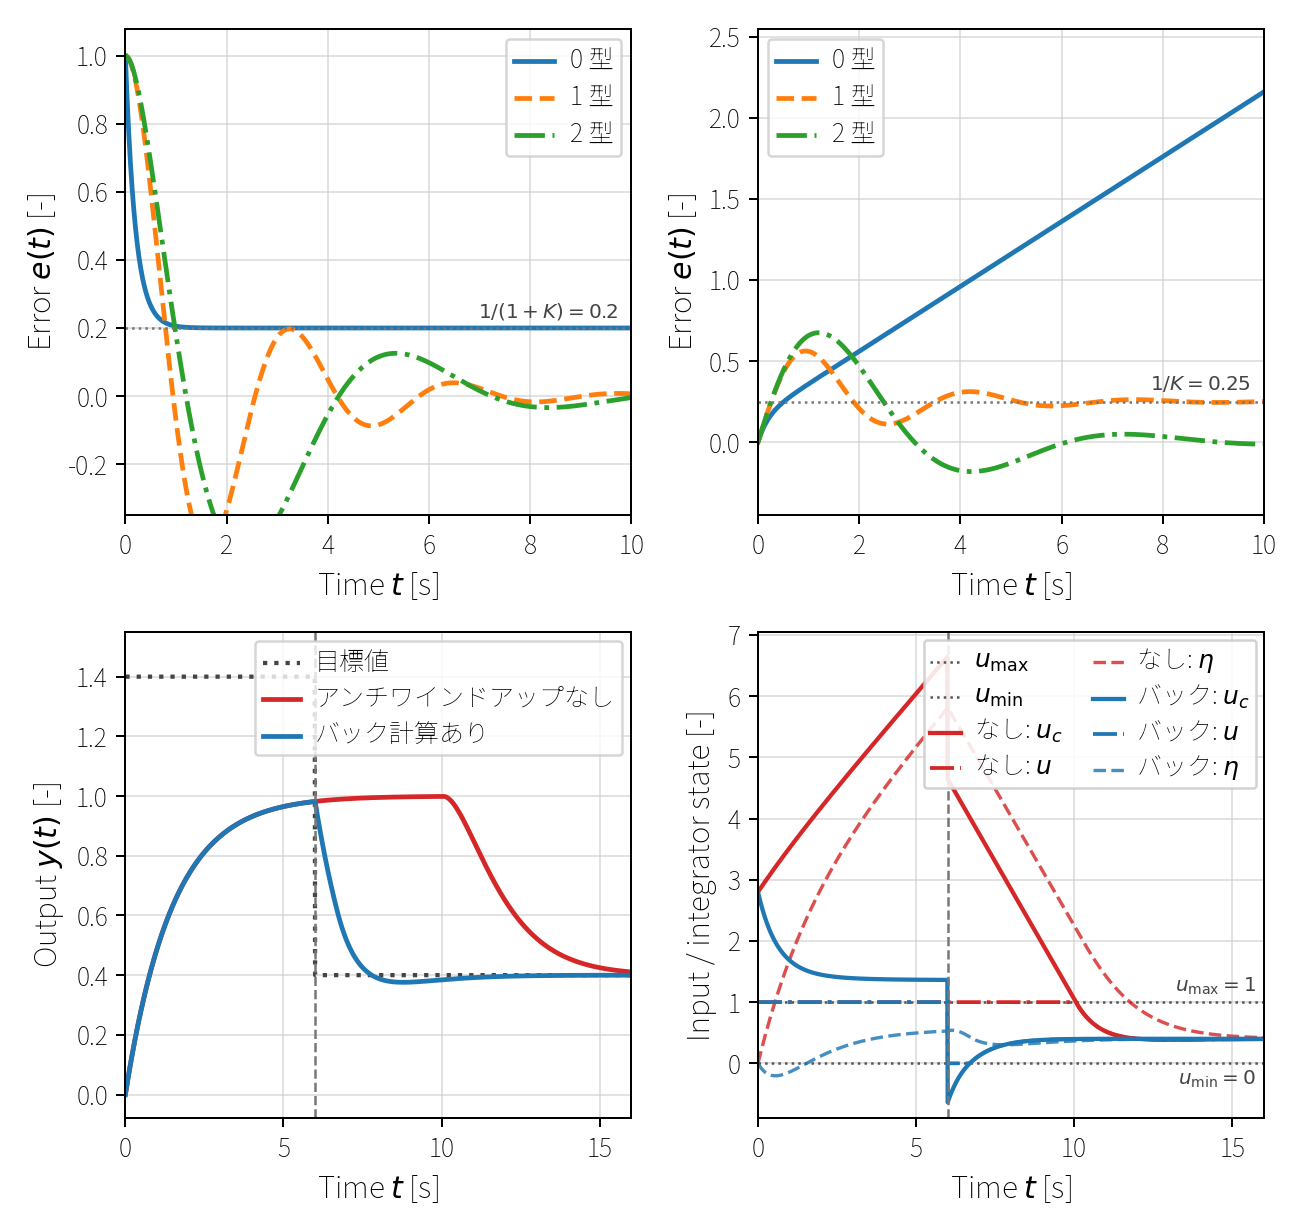
\includegraphics[width=0.96\linewidth,bb=0 0 1296 1224]{figures/classical_design_examples.png}
\caption{系の型による定常偏差と、飽和時の PI 制御におけるアンチワインドアップ効果。上段は $L_0(s)=4/(s+1)$、$L_1(s)=4/\{s(s+1)\}$、$L_2(s)=4(s+1)/\{s^2(s+4)\}$ の単位負帰還を同じ入力で比較し、型が上がると追従できる基準入力の次数が一つずつ上がることを示す。下段は $P(s)=1/(1.5s+1)$、$K_P=2.0$、$K_I=1.5$、$0\leq u\leq1$ の PI 制御で、バック計算が飽和中の積分状態を入力制約に合わせて戻すことを示す。}
\label{fig:classical-design-examples}
\end{figure}

\begin{practice}[定常偏差とアンチワインドアップの波形確認]
\wfig{classical-design-examples} の上段について、$K=4$ を用いて $0$ 型のステップ偏差 $1/(1+K)$ と $1$ 型のランプ偏差 $1/K$ を計算し、図中の水平破線と対応させよ。下段については、$t=6\,\mathrm{s}$ の直後に、アンチワインドアップなしの $\eta$ とバック計算ありの $\eta$ のどちらが $u_{\max}=1$ から大きく離れているかを読み取り、\weq{back-calculation-discrete} の補正項 $T_s(u_k-v_k)/T_t$ がその差を小さくする向きを説明せよ。
\end{practice}

\subsubsection{バンプレス切替}

手動運転から自動制御へ切り替えるとき、制御器内部の積分状態が現在の手動入力と整合していないと、切替瞬間に $u_c$ が段差を持つ。この段差を避けることをバンプレス切替という。切替時刻を $t_0$、手動で実際に入っている入力を $u_m(t_0)$ とする。二自由度 PID の内部状態は
\begin{equation}
  \eta(t_0^+)=u_m(t_0)-u_b
  -K_P\{\beta r(t_0)-y(t_0)\}
  -K_D\{\gamma d_r(t_0)-d_y(t_0)\}
  \label{eq:bumpless-initialization}
\end{equation}
に初期化する。これを \weq{two-degree-pid} に代入すると、切替直後の計算入力は $u_c(t_0^+)=u_m(t_0)$ となる。

手動運転中にも内部状態を追従させておく方法もある。手動入力に整合する積分状態を
\begin{equation}
  \eta_{tr}=u_m-u_b
  -K_P(\beta r-y)
  -K_D(\gamma d_r-d_y)
\end{equation}
と定義し、手動中は
\begin{equation}
  \dot{\eta}=\frac{1}{T_b}(\eta_{tr}-\eta)
\end{equation}
で更新する。$T_b$ は追従時定数で、単位は秒である。離散時間では後退オイラー近似により
\begin{equation}
  \eta_k=
  \frac{T_b}{T_b+T_s}\eta_{k-1}
  +\frac{T_s}{T_b+T_s}\eta_{tr,k}
\end{equation}
と更新できる。自動制御へ切り替える瞬間に $\eta_k=\eta_{tr,k}$ と代入してもよい。$T_b$ を十分小さくすれば、切替時に \weq{bumpless-initialization} とほぼ同じ状態になり、手動入力から自動入力へ連続に移れる。
